%------------------------------------------------------------------------------------------------------------------%
% Präambel 

% Dokumenteinstellungen
\documentclass[a4paper,11pt]{scrartcl}

% Packages
\usepackage[table,xcdraw]{xcolor}
\usepackage{graphicx}
\usepackage[utf8]{inputenc}
\usepackage[ngerman]{babel}
\usepackage[T1]{fontenc}
\usepackage{geometry}
\usepackage[headsepline, footsepline]{scrpage2}
\usepackage{pdfpages}
\usepackage{graphicx}
\usepackage{float}
\usepackage{acronym}
\usepackage[hidelinks]{hyperref} % Referenzen im Text erzeugen
\usepackage[style=ieee, sorting=none, dashed=false]{biblatex}
\usepackage{setspace}
\usepackage{tikz}
\usepackage{enumitem}
\usepackage{svg}
\usepackage{amsmath}
\usepackage[font={small}]{caption}
\usepackage{booktabs}
\usepackage{listings}
\usepackage{setspace}
\usepackage{subfigure}
\bibliography{Literature.bib}


% Zeilenabstand
\makeatletter
\newcommand{\MSonehalfspacing}{%
	\setstretch{1.44}%  default
	\ifcase \@ptsize \relax % 10pt
	\setstretch {1.448}%
	\or % 11pt
	\setstretch {1.399}%
	\or % 12pt
	\setstretch {1.433}%
	\fi
}
\makeatother
\MSonehalfspacing

% Seitenränder
\geometry{
	left=3cm,
	right=3cm,
	top=3cm,
	bottom=4cm,
	bindingoffset=5mm
}

% Einzug vor Absatz
\parindent0mm

% Kopf- und Fußzeile
\pagestyle{scrheadings} % Aktiviere Kopf- und Fußzeilen

\ihead{\headmark}
\chead{}
\ohead[\pagemark]{\pagemark}

\automark[section]{chapter}

\cfoot{}

% Metadaten
\title{Digital Image Processing}
\author{Adam Mahmoud, Michael Wimmer, Philipp Kronser}
\date{\today}

%------------------------------------------------------------------------------------------------------------------%
% Begin eigentliches Dokument
\begin{document}
%------------------------------------------------------------------------------------------------------------------%
% Titelseite
\begin{titlepage}
	\centering
	
\includegraphics[width=0.5\textwidth]{Figures/LogoHM}\par
	\vspace{1cm}
	{\scshape\LARGE Hochschule München \par}
	\vspace{1cm}
	{\scshape\Large Digital Image Processing\par}
	\vspace{1.5cm}
	{\huge\bfseries Image Stitching and Point Cloud Generation from Smartphone Pictures\par}
	\vspace{2cm}
	Verfasst von\par
	{\Large\itshape Adam Mahmoud\\ Michael Wimmer \\ Philipp Kronser\par}
	\vfill
	Vorgelegt bei\par
	Prof. Dr. Claudius \textsc{Schnörr}
	
	\vfill
	
	% Bottom of the page
	{\large \today\par}
\end{titlepage}

\clearpage
%------------------------------------------------------------------------------------------------------------------%
% Abkürzungsverzeichnis
\section*{Abkürzungsverzeichnis} %Abkürzungsverzeichnis 

\addcontentsline{toc}{section}{Abkürzungsverzeichnis}

\begin{acronym}[VeryLongAndUsefullStuff]
	\acro{BOM}{Bill of Materials}
	\acro{BTC}{Bitcoin}
	\acro{CAD}{Computer-Aided Design}
	\acro{DApp}{Dezentralisierte Apps}
	\acro{DRM}{Design Research Methodology}
	\acro{ETH}{Ether}
	\acro{ERP}{Enterprise Ressource Planning}
	\acro{EVM}{Ethereum Virtual Machine}
	\acro{PDM}{Product Data Management}
	\acro{PLM}{Product Lifecycle Management}
	\acro{PoS}{Proof of Stake}
	\acro{PoW}{Proof of Work}
	\acro{STEP}{Standard for the exchange of product model data}
\end{acronym}

\clearpage

%------------------------------------------------------------------------------------------------------------------%
% Inhaltsverzeichnis 
\begin{spacing}{1.25}
	\tableofcontents
\end{spacing}

%{\small\tableofcontents}

\clearpage
%------------------------------------------------------------------------------------------------------------------%


% Weitere Kapitel
% Kapitel 0

\section{Einleitung}

%Aktuelle Entwicklungen -> neue Herausforderungen -> Baaam, da ist die Blockchain Anwendung!

\subsection{Motivation und Ziel der Arbeit}

\par \bigskip
Lalala




\subsection{Aufbau der Arbeit}

\par \bigskip
Lalala

\clearpage
% Kapitel 1

\section{Feature Erkennung und Korrespondenzanalyse}
\label{kap:FeatureErkennungUndKorrespondenzanalyse}

\subsection{Feature Erkennung}
\label{kap:FeatureErkennung}

\subsection{Korrespondenzanalyse}
\label{kap:Korrespondenzanalyse}


\clearpage

% Kapitel 2
\newcommand\todo[1]{
\newline
\textcolor{red}{#1}
}

\section{Image Stitching}
\label{sec:ImageStitching}
In dieser Aufgabe sollen überlappende Bilder, welche von einem Kamerastandpunkt aufgenommen wurden, automatisch zu einem Panoramabild zusammengeflickt werden. In unserer Implementierung werden nur zwei Bilder zusammengeflickt. Der Algorithmus kann mit einigen Anpassungen für beliebig große Bildfolgen gelten.

\begin{figure}[ht]
    \centering
    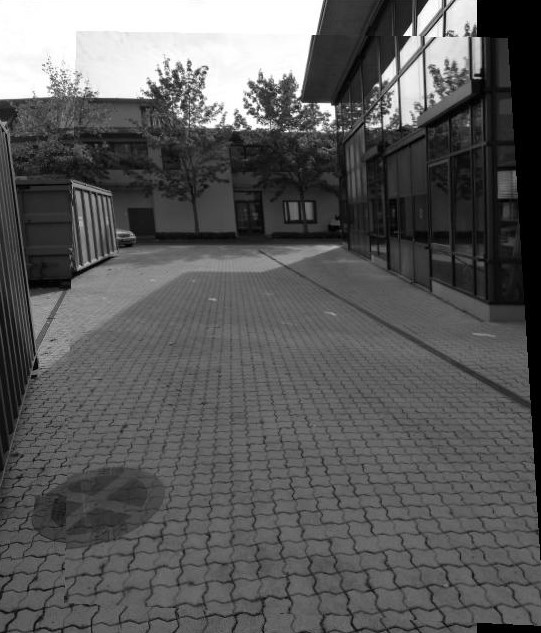
\includegraphics[width=0.49\textwidth]{FiguresIS/ergebnis.jpg}
    \caption{Ergebnis des eigenen Algorithmus beim stitching von zwei Bildern}
\end{figure}

\subsection{Algorithmus}
In diesem Kapitel wird ein Überblick über den Algorithmus gegeben, der die Bilder zusammenflickt. Die Details der Unteralgorithmen werden in den folgenden Kapiteln genauer erklärt. Die Vorgehensweise ist an \cite{Richard2000} orientiert. Zuerst müssen die Bilder geladen werden. Sie werden in Graustufenbilder umgewandelt, da die darauf folgenden Algorithmen auf 1-kanalige Bilder ausgelegt sind.
Auf beiden Bildern werden nun mithilfe des Harris Corner Detektors markante Punkte ermittelt. (\ref{kap:FeatureErkennung}). Nun werden die markanten Punkte auf Bild 1 und Bild 2 mithilfe des feature matching miteinander verglichen, um korrespondierende Punkte festzustellen. Diese werden als Korrespondenzen oder matches bezeichnet. Eine genauere Erläuterung zum feature matching befindet sich im Kapitel \ref{kap:Korrespondenzanalyse} Bei den Korrespondenzen kann man davon ausgehen, dass es sich um den gleichen Punkt des dargestellten Objekts auf beiden Bildern handelt.
Aus den Korrespondierenden Punkten kann dann im RANSAC verfahren eine Homographiematrix berechnet werden, welche die Transformation zwischen den Bildern beschreibt. Im Folgenden wird sie auch $H$-Matrix genannt. Das bedeutet, dass man mithilfe dieser Matrix für jeden Punkt in einem der beiden Bilder seine Position im anderen Bild berechnen kann.  In diesem Beispiel wurde die $H$-Matrix für eine projektive Transformation berechnet
Anschließend werden die beiden Bilder zusammengefügt indem das zweite Bild mit der $H$-Matrix transformiert wird.

\subsection{Transformation eines Punktes}
Um einen Punkt $p$ mithilfe einer gegebenen projektiven Transformationsmatrix $H$ zu transformieren wird dieser mit der Matrix multipliziert. Dazu muss der Punkt in homogenen Koordinaten $[p1 p2 w]$ angegeben werden. In unserer Implementierung brauchen wir 2-dimensionale Koordinaten. Deswegen muss gelten w=1. Das Vorgehen für eine Transformation ist also folgendes:
 $$p H=p‘$$
$$p`=p`/w`$$
Das Ergebnis der Matrixmultiplikation wird jedes Mal durch den inversen Streckungsfaktor w geteilt sodass $p`$ in Bildkoordinaten gegeben ist

\subsection{Berechnung der Transformationsmatrix }
Hat man einen Punkt $x$ gegeben als Zeilenvektor und multipliziert diesen mit einer Transformationsmatrix dann entsteht ein Punkt $p‘$, der nach Vorgaben der Matrix transformiert wurde. Zwischen diesen Punkten herrscht also die Beziehung
				$$x H =x‘$$
In diesem Anwendungsfall wird in der zweidimensionalen Ebene gearbeitet. Für die Transformation wird die projektive Transformation angewendet. Translation und Rotation allein wären nicht ausreichend, um die Bilder gut zusammen zu flicken. Die affine Transformation wäre genug für Bilder, deren Inhalt weit vom Betrachter entfernt ist. Bei unseren Bildern ist der Bildinhalt so nah, dass eine projektive Transformation nötig ist, um das Bild richtig zu verzerren. Für die projektive Transformation muss eine 3x3 Matrix bestimmt werden, die in Abbildung \ref{img:42} gezeigt wird.

\begin{figure}[ht]
    \centering
    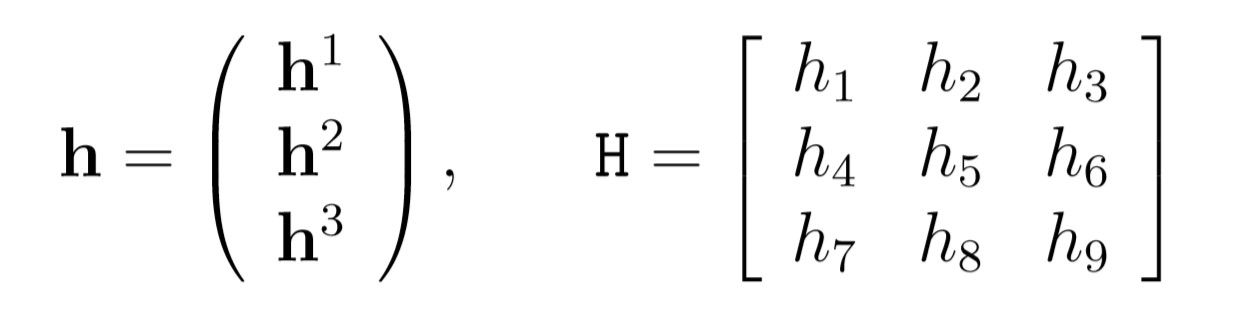
\includegraphics[width=0.49\textwidth]{FiguresIS/42.jpg}
    \caption{\cite{Richard2000} Rechts befindet sich die komplette $H$-Matrix mit allen Elementen. Links die gleiche Matrix dargestellt als Vektoren, welche jeweils eine Zeile der Matrix repräsentieren.}
    \label{img:42}
\end{figure}

Um zweidimensionale Punkte mit dieser Matrix multiplizieren zu können müssen diese in die homogene Darstellung gebracht werden. In dieser Darstellung ist der Punkt als Vektor mit einem inversen Streckungsfaktor w bestimmt. 
				$$[x1, x2, w]$$
Die $H$ Matrix muss nun aus den Punktkorrespondenzen bestimmt werden. Damit Sie vollständig bestimmt ist müssen mindestens vier Punktkorrespondenzen vorhanden sein.
Das Kreuzprodukt aus zwei gleichen Vektoren ist Null. Diese Eigenschaft macht man sich zu Nutze, um eine Lineare Lösung für die $H$-Matrix zu finden. Man kann also schreiben:
			$$ x‘ \times H x=0$$
Jede j-e Zeile der Matrix kann als $h_j^T$ bezeichnet werden dann kann man das Kreuzprodukt ausschreiben wie in Abbildung \ref{img:40}.

\begin{figure}[ht]
    \centering
    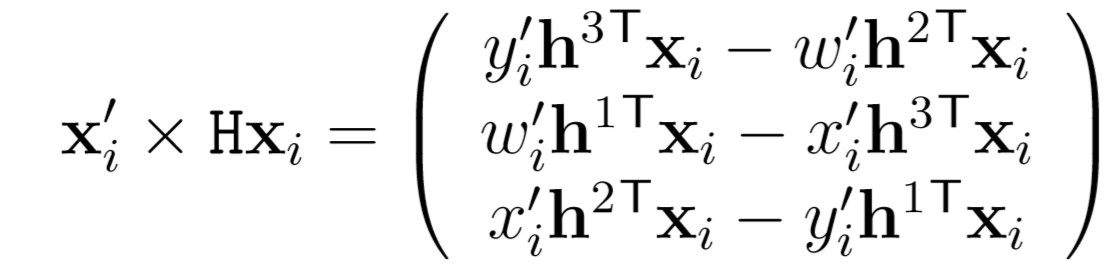
\includegraphics[width=0.49\textwidth]{FiguresIS/40.jpg}
    \caption{\cite{Richard2000}}
     \label{img:40}
\end{figure}

Da $h_j^T\times x=x^T\times h_j$ ergibt das drei Gleichungen.  Man kann sie in Matrizenform schreiben wie in Abbildung \ref{img:41}.
 
\begin{figure}[ht]
    \centering
    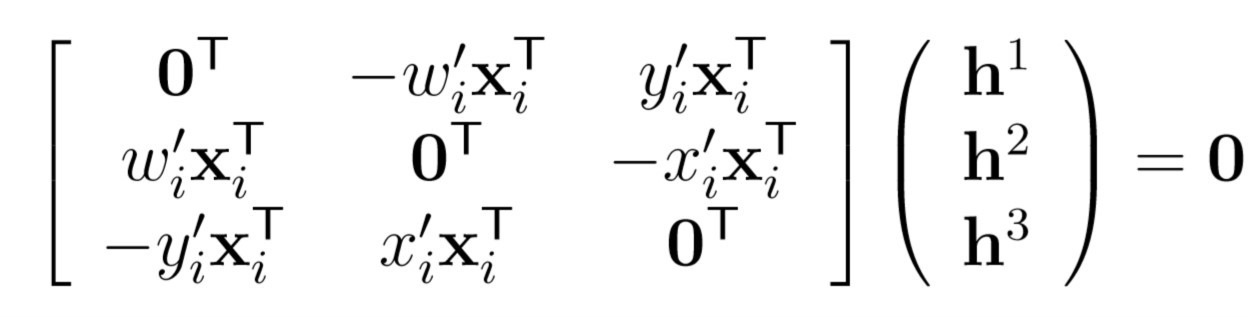
\includegraphics[width=0.49\textwidth]{FiguresIS/41.jpg}
    \caption{\cite{Richard2000}}
     \label{img:41}
\end{figure}


Von den drei Gleichungen sind nur zwei linear unabhängig. Die dritte Zeile ergibt sich aus einer Linearkombination von den beiden anderen. Die Gleichungen werden dann wie in Abbildung \ref{img:43} gezeigt.

\begin{figure}[ht]
    \centering
    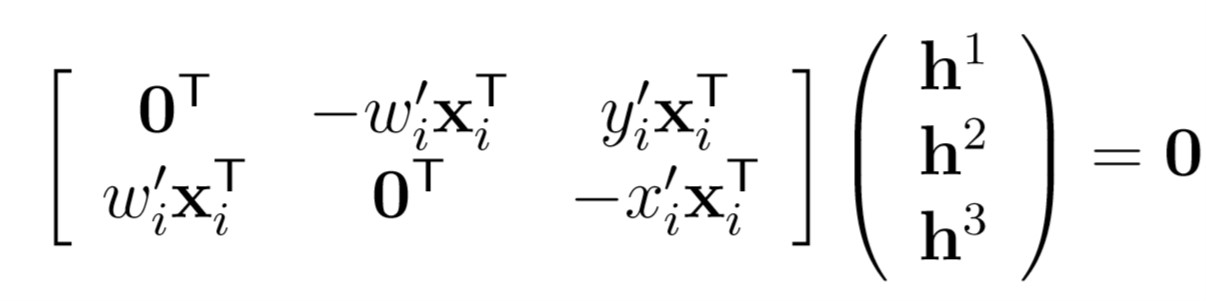
\includegraphics[width=0.49\textwidth]{FiguresIS/43.jpg}
    \caption{\cite{Richard2000}}
     \label{img:43}
\end{figure}

Diese Gleichungen gelten für alle Punktkorrespondenzen in homogener Darstellung. Wählt man den inversen Streckungsfaktor w als 1 dann vereinfacht sich die Gleichung und die Punkte können als:
			$$[x, y, 1]$$
Dargestellt werden. Wobei $x$ und $y$ die Koordinaten aus dem Bild sind.

\subsection{Inhomogene Lösung}
Bis jetzt besteht das Gleichungssystem aus acht linear unabhängigen Gleichungen und neun unbekannten $h_j$. Für die inhomogene Lösung wird ein Eintrag von $h$ zu $h_j$=1 gesetzt. Das ist zulässig da die $H$-Matrix bis auf einen Skalierungsfaktor bestimmt ist und dieser beliebig gewählt werden kann. In unserer Implementierung wurde $h_9=1$ gesetzt. Somit bleibt ein Gleichungssystem mit acht Gleichungen und acht unbekannten übrig.
Dieses Gleichungssystem wird mithilfe einer Singulärwertzerlegung gelöst. Dazu wir die gesamte Matrix, die sich aus den Gleichungen ergibt in die Matrizen $U$, $D$ und $V$ zerlegt. Wobei $U$ und $V$ orthogonale Matrizen sind und $D$ eine Diagonalmatrix bestehend aus den Singulärwerten. Die Zerlegung wird so gemacht, dass die Einträge der Diagonalmatrix vom größten zum kleinsten sortiert sind. Die Lösung ist der Singulärvektor mit dem kleinsten Singulärwert. Das entspricht wegen der Sortierung der letzten Spalte der Matrix $V$. Somit ist $h$ gelöst und muss wieder in $H$ umgewandelt werden indem die Einträge $h_1$, $h_2$ und $h_3$ gestapelt werden zu $H$.

\subsection{RANSAC Verfahren}
Bei der Suche von markanten Punkten in den Bildern und beim feature matching entstehen in einer Anwendung mit Fotos oft viele Fehler. Einerseits können die markanten Punkte z.B. aufgrund von Unschärfe eine ungenaue Position haben und andererseits können die Korrespondenzen falsch sein. Das passiert vor allem wenn das Bild wiederholende Strukturen (z.B. Gehwegplatten) hat. Dann kann es sein, dass Features verwechselt werden. Zusätzlich zu diesen beiden Fehlern spielt die Verzeichnung aufgrund der Krümmung der Kameralinse ebenfalls eine Rolle. Dadurch kann passieren, dass eine $H$-Matrix, die aus 4 matches in einem Teil des Bildes berechnet wurde zwar für diesen Teil gut gilt, allerdings passt dann der Rest der beiden Bilder nicht korrekt zusammen.
Um diesen Fehlern entgegenzuwirken wird mithilfe des RANSAC Algorithmus die $H$-Matrix gefunden, die möglichst fehlerfrei ist. RANSAC steht für RANdom SAmple Consensus. Der Algorithmus wird als robuste Schätzung bezeichnet, da er trotz einer großen Anzahl an fehlerhaften Samples ein gutes Ergebnis erreichen kann. Für die Schätzung der $H$ Matrix aus den matches von zwei Bildern sieht der Algorithmus wie folgt aus:

\begin{itemize}
    \item Für n Wiederholungen:

    \begin{itemize}
        \item Es werden vier zufällige matches aus dem Set ausgewählt
        \item Aus diesen wird eine $H$-Matrix berechnet.
        \item Für jeden anderen match wird die geometrische Distanz berechnet. Jeder match dessen geometrische Distanz kleiner als der Mindestwert ist gilt als inlier.
    \end{itemize}
    
    \item Für beliebige Widerholungen:
    
    \begin{itemize}
        \item Die $H$-Matrix mit den meisten inliern wird ausgewählt.
        \item Die $H$-Matrix wird nochmal berechnet unter Verwendung aller inlier.
    \end{itemize}
    
\end{itemize}


Somit wird eine $H$-Matrix ausgewählt, die für möglichst viele der matches gilt. Der Algorithmus ist so robust, dass sogar bei fehlerraten von über 50\% gute Ergebnisse erreicht werden können. Das setzt voraus, dass keine systematischen Fehler auftreten, wie beispielweise eine fälschliche Verschiebung vieler matches um einen bestimmten Wert oder eine Rotation vieler matches. In diesem Fall wird der Algorithmus die $H$-Matrix falsch optimieren. Diese Fehler können nur sehr selten auftreten, wenn das Bild sich sehr wiederholende und ähnliche Strukturen aufweist. Man kann solche Fehler sehr leicht am Ergebnisbild erkennen. Abhilfe kann hier dann nur ein komplexerer feature matching Algorithmus schaffen, der die Strukturen besser unterscheiden kann.

\subsubsection{Parameter im RANSAC Verfahren}
Im RANSAC Verfahren werden für zufällige Punktekombinationen $H$-Matrizen berechnet. Der Zufall ist deswegen wichtig, da die Anzahl der Kombinationen mit der vierten Potenz der Anzahl von matches steigt. Eine testweise Implementierung eines “Brute Force Sample Consensus” der alle möglichen $H$-Matrizen berechnet und die beste auswählt, dauert bereits bei einer kleinen Anzahl von 17 matches etwa fünf Minuten auf meinem Rechner.Eine ähnliche Menge an matches dauert beim RANSAC nur Bruchteile von Sekunden. Durch zufällige Auswahl der Punkte soll sichergestellt werden, dass mit der  Wahrscheinlichkeit $p$ eine $H$-Matrix berechnet wird, die ein inlier ist, also hinreichend genau ist. Um das sicherstellen zu können muss eine Mindestanzahl an 4-Punkt-Kombinationen geprüft werden. Nimmt man an dass $s$ die Anzahl der Punkte ist, die für die Berechnung einer $H$-Matrix benötigt werden und $\eta$ die geschätzte Menge an Ausreißern dann lässt sich die Mindestanzahl über die folgende Formel berechnen:
$$N=log(1-p)/log(1-(1-\eta)^s)$$
Ein weiterer Parameter, der für den RANSAC festgelegt werden muss ist die Schwelle für die geometrische Distanz, ab der ein Punkt als inlier gilt. Diese Schwelle sollte theoretisch $5.99*\sigma ^2$ betragen, da aber Sigma am Anfang der Berechnung nicht gegeben ist wurde die Schwelle durch probieren auf 4 festgelegt.

\subsubsection{Geometrische Distanz}
Um messbar zu bestimmen wie gut eine $H$-Matrix sich für eine Bildtransformation eignet, kann man die matches verwenden. Jedes Punktepaar einer Korrespondenz, besteht aus dem Punkt $x$ auf dem ersten Bild und dessen Entsprechung $y$ auf dem zweiten Bild. Die $H$-Matrix beschreibt die Transformation von $x$ nach $y$. Wären die matches und die Matrix fehlerfrei dann würde exakt gelten:
$$x H= y$$
Aufgrund von Ungenauigkeiten und Fehlern wird $x$ durch die Transformation mit $H$ abgebildet auf einen Punkt $x‘$, der von $y$ um den Abstand $d$ entfernt ist. Beim geometrischen Abstand wird einmal $x$ zu $x‘$ transformiert und einmal $y$ zu $ y‘$ rücktransformiert und es wird der Abstand zwischen den sich ergebenden Punkten und den tatsächlichen gebildet. Dieser Abstand wird dann quadratisch addiert. So ergibt sich der geometrische Abstand. Dies Summe über alle Punkte entspricht dann dem geometrischen Fehler (Siehe Abb. \ref{img47}). 

\begin{figure}[ht]
    \centering
    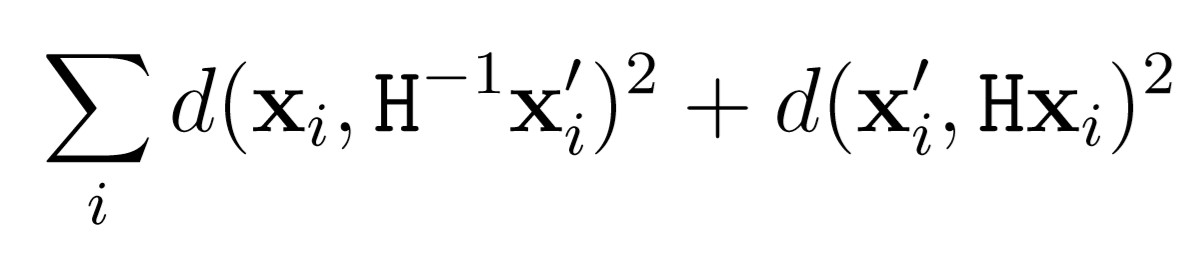
\includegraphics[width=0.49\textwidth]{FiguresIS/47.jpg}
    \caption{\cite{Richard2000}}
     \label{img:47}
\end{figure}

Über diesen kann dann bestimmt werden ob ein Punkt für eine $H$-Matrix ein inlier ist oder nicht. Berechnet man den Erwartungswert und die Standartabweichung der geometrischen Distanz für alle Bildkorrespondenzen für eine $H$-Matrix so erhält man ein Maß für die Güte dieser $H$-Matrix.

\subsection{Bildtransformation}
Sobald die $H$-Matrix fertig ist müssen die Bilder überlagert werden. Dazu muss das zweite Bild mit der $H$-Matrix transformiert werden. Beim Transformieren eines ganzen Bildes muss jedes Pixel an seine neue Position gebracht werden. Dabei kann es auftreten, dass es im neuen Bild ungefüllte Positionen, also Lücken gibt. Um dem entgegenzuwirken wird bilineare Interpolation verwendet. Ein weiteres Problem, das entstehen kann ist, dass das transformierte Bild sich im negativen Bereich befindet. Das ist von der Datenstruktur unmöglich abzuspeichern. Das folgende Vorgehen ist so gemacht, dass beide oben beschriebene Probleme nicht auftreten.
Zuerst wird das fertige gemeinsame Bild als Matrix von Nullen festgelegt. Dazu werden die Eckpunkte des zweiten Bildes transformiert. Aus Den Eckpunkten des ersten Bildes und denen des transformierten zweiten Bildes lässt sich die resultierende Bildgröße berechnen. Sind die Punkte des transformierten zweiten Bildes negativ in einer oder beiden Dimensionen, so ist das der Offset, der auf beide Bilder addiert wird und diese in positive Richtung verschiebt.
Nun werden beide Bilder auf den canvas übertragen. Das Vorgehen ist so:


\begin{itemize}
\item Für alle Pixel $p`$ innerhalb des transformierten Bildbereichs auf dem canvas:
\item Transformiere $p`$ zurück zu $p$ mit der inversen von H
\item Wenn $p$ innerhalb des nicht transformierten Bildes liegt:
\begin{itemize}
    \item Führe bilineare Interpolation zwischen den umliegenden Pixeln von $p$ aus
    \item  Schreibe das Ergebnis in $p`$Auf diese Weise können wird das resultierende Gesamtbild aus  dem negativen Bereich geschoben und es können niemals Lücken zwischen den Pixeln entstehen.
\end{itemize}

\end{itemize}

Auf diese Weise können wird das resultierende Gesamtbild aus dem negativen Bereich geschoben und es können niemals Lücken zwischen den Pixeln entstehen. Es muss jedoch darauf hingewiesen werden, dass diese Art von Bildtransformation deutlich langsamer ist als entsprechende Bibliotheksfunktionen, da solche Operationen wie Transformation und bilineare Interpolation normalerweise durch die Grafik-Pipeline erledigt werden, welche das hardwarebeschleunigt ausführt.

\clearpage
\section{3-D Punktwolke}
\label{3-D Punktwolke}
In dieser Aufgabe soll aus einer Reihe von Bildern eines Objekts, welche von verschiedenen Kamerastandpunkten aufgenommen wurden, eine 3D Punktwolke des Objekts berechnet werden. 

\subsection{Algorithmus}
In diesem Kapitel wird der gesamte Algorithmus erklärt, der von der Bildserie zur 3D Punktwolke führt. Er enthält einige komplexe Unteralgorithmen die in den nächsten Kapiteln erläutert werden. Die grobe Vorgehensweise ist an \cite{Mathworks} angelehnt.
Zunächst müssen die Bilder des Objekts geladen werden. Dabei ist es wichtig dass sie in der richtigen Reihenfolge geladen werden, da aufeinanderfolgende Bilder eine Überlappung von mindestens 50\% haben müssen. Außerdem müssen die Bilder in Grauwertbilder umgewandelt werden, da die darauffolgenden Algorithmen nur mit 1-kanaligen Bildern umgehen können. Zusätzlich müssen die Kameraparameter der Kamera, mit denen die Bilder aufgenommen wurden, geladen werden. Die Ermittlung der Kameraparameter wird in Kapitel \ref{sec:Kamerakalibrierung} beschrieben.
Nun wird das erste Bild verarbeitet, indem es über die Funktion undistortImage und die Kameraparameter verzeichungsfrei (s. Kapitel \ref{sec:Kamerakalibrierung}) gemacht wird.
Als nächstes werden auf dem ersten Bild markante Punkte über den Harris Corner Detector (s. Kapitel \ref{kap:FeatureErkennungUndKorrespondenzanalyse}) ermittelt. Nun wird der erste Kamerastandpunkt, er ist der Referenzstandpunkt im Nullpunkt mit der Einheitsmatrix als Orientierung, mitsamt der markanten Punkte in eine Datenstruktur mit dem Namen ViewSet gespeichert. Diese speichert alle Parameter eines Kamerastandpunkts und ordnet diesen eine ID zu. Beim ersten Bild ist dies die ID 1.
Es folgt eine Schleife die über alle Bilder iteriert. Mit dem nächsten Bild wird nun analog zum ersten Verfahren, es wird verzeichnungsfrei gerechnet und seine markanten Punkte werden ermittelt. Nun werden aber Punkte zwischen dem vorigen und dem gerade in der Schleife untersuchten Bild ermittelt die in beiden Bildern vorkommen. Solche Punkte werden als korrespondierende Punkte oder Matches bezeichnet. Die genaue Erläuterung der Berechnung von Matches folgt in Kapitel \ref{kap:FeatureErkennungUndKorrespondenzanalyse}.
Mit diesen ermittelten Matches kann nun eine sogenannte Fundamentalmatrix berechnet werden. Diese enthält Informationen über die intrinsischen und extrinsischen Kameraparameter. Das genaue Vorgehen zur Berechnug der Fundamentalmatrix sowie deren Eigenschaften werden in Kapitel \ref{sec:Schätzen der Fundamentalmatrix} erläutert. 
Aus der Fundamentalmatrix kann durch Multiplikation der intrinsischen Kameraparameter beider Kameras (hier identisch da gleiche Kamera) die Essentielle Matrix berechnet werden, die nur noch Informationen über die extrinsischen Kameraparameter enthält. Im nächsten Schritt kann nun aus der Essentiellen Matrix die Lage und Orientierung der Kameras zueinander ermittelt werden. (siehe Kapitel \ref{sec:Schätzen der Kamerapose aus der Fundamentalmatrix}).
Die berechnete Kamerapose sowie die Matches werden mit der nächsten ID in die ViewSet  Datenstruktur gespeichert. Da zwischen den Bildern jeweils nur relative Posen berechnet werden, müssen diese zuvor noch mit der Position und Orientierung des vorigen Standpunkts verechnet werden. 
Im letzten Schritt innerhalb der Schleife wird nun das aktuelle Bild zum vorigen Bild, sodass zwischen diesem und dem nächsten wieder eine Korrespondenzanalyse sowie die Ermittlung der Kamerapose berechnet werden kann.
Sind alle Kameraposen und deren Matches im ViewSet gespeichert kann nun eine Triangulation der Matches stattfinden. Dazu werden mit der Funktion findTracks Punkte ermittelt die in mehreren Bildern (mind. 2) auftauchen. Über diese Tracks wird eine Triangulation wie im Kapitel \ref{sec:Triangulation} beschrieben durchgeführt. Ergebnis sind Punkte im 3D Raum die zum Schluss noch geplottet werden.
Das gesamte Vorgehen wird hier nocheinmal im Pseudocode zusammengefasst.
\begin{figure}[ht]
    \centering
    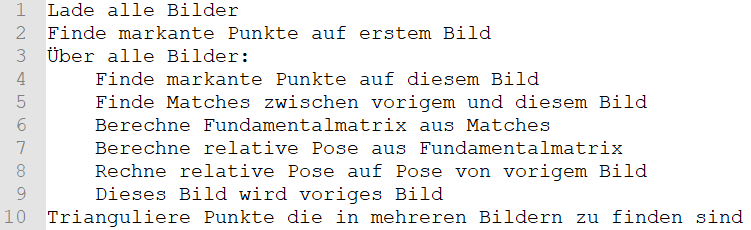
\includegraphics[scale=0.75]{Figures/Pseudocode.PNG}
    \caption{Pseudocode}
\end{figure}

\subsection{Kamerakalibrierung}
\label{sec:Kamerakalibrierung}
Die Kalibrierung der Kamera ist wichtig, da die Abbildung jeder Kamera ein wenig anders ist. So unterscheiden sich zum Beispiel die Brennweiten von Gerät zu Gerät geringfügig und jede Kamera hat ihre eigenen Verzeichnungsfehler.
Es gibt zwei Arten von Verzeichnungsfehlern, die tangentiale und die radiale. Die radiale Verzeichnung entsteht durch die Krümmung der Linse bzw. kleine Unebenheiten die bei der Produktion entstanden sind. Die tangentiale Verzeichnung entsteht dadurch dass der Fotochip nicht exakt parallel zur Linse eingebaut wurde. Die Folgenden Bilder zeigen die Auswirkungen von tangentialer und radialer Verzeichnung.\cite{Verlag}

\begin{figure}[ht]
\centering
    \subfigure {
    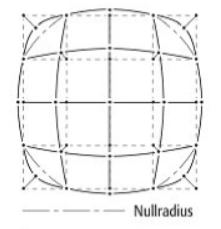
\includegraphics[scale=0.5]{Figures/RadialeVerzeichnung.PNG}
    }
    \subfigure{
    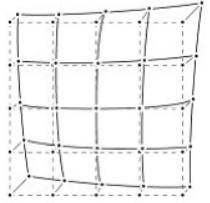
\includegraphics[scale=0.5]{Figures/tangentialeVerzeichnung.PNG}
    }
    \caption{Auswirkung von Verzeichnung (links radial, rechts tangential) \cite{Verlag}}
\end{figure}

Matlab bietet eine Applikation die aus Bildern von einem Kalibrierungsboard die Kameraparameter schätzt. Dazu muss das Board aus vielen verschiedenen Positionen (ca. 20) fotographiert werden. 
\begin{figure}[ht]
    \centering
    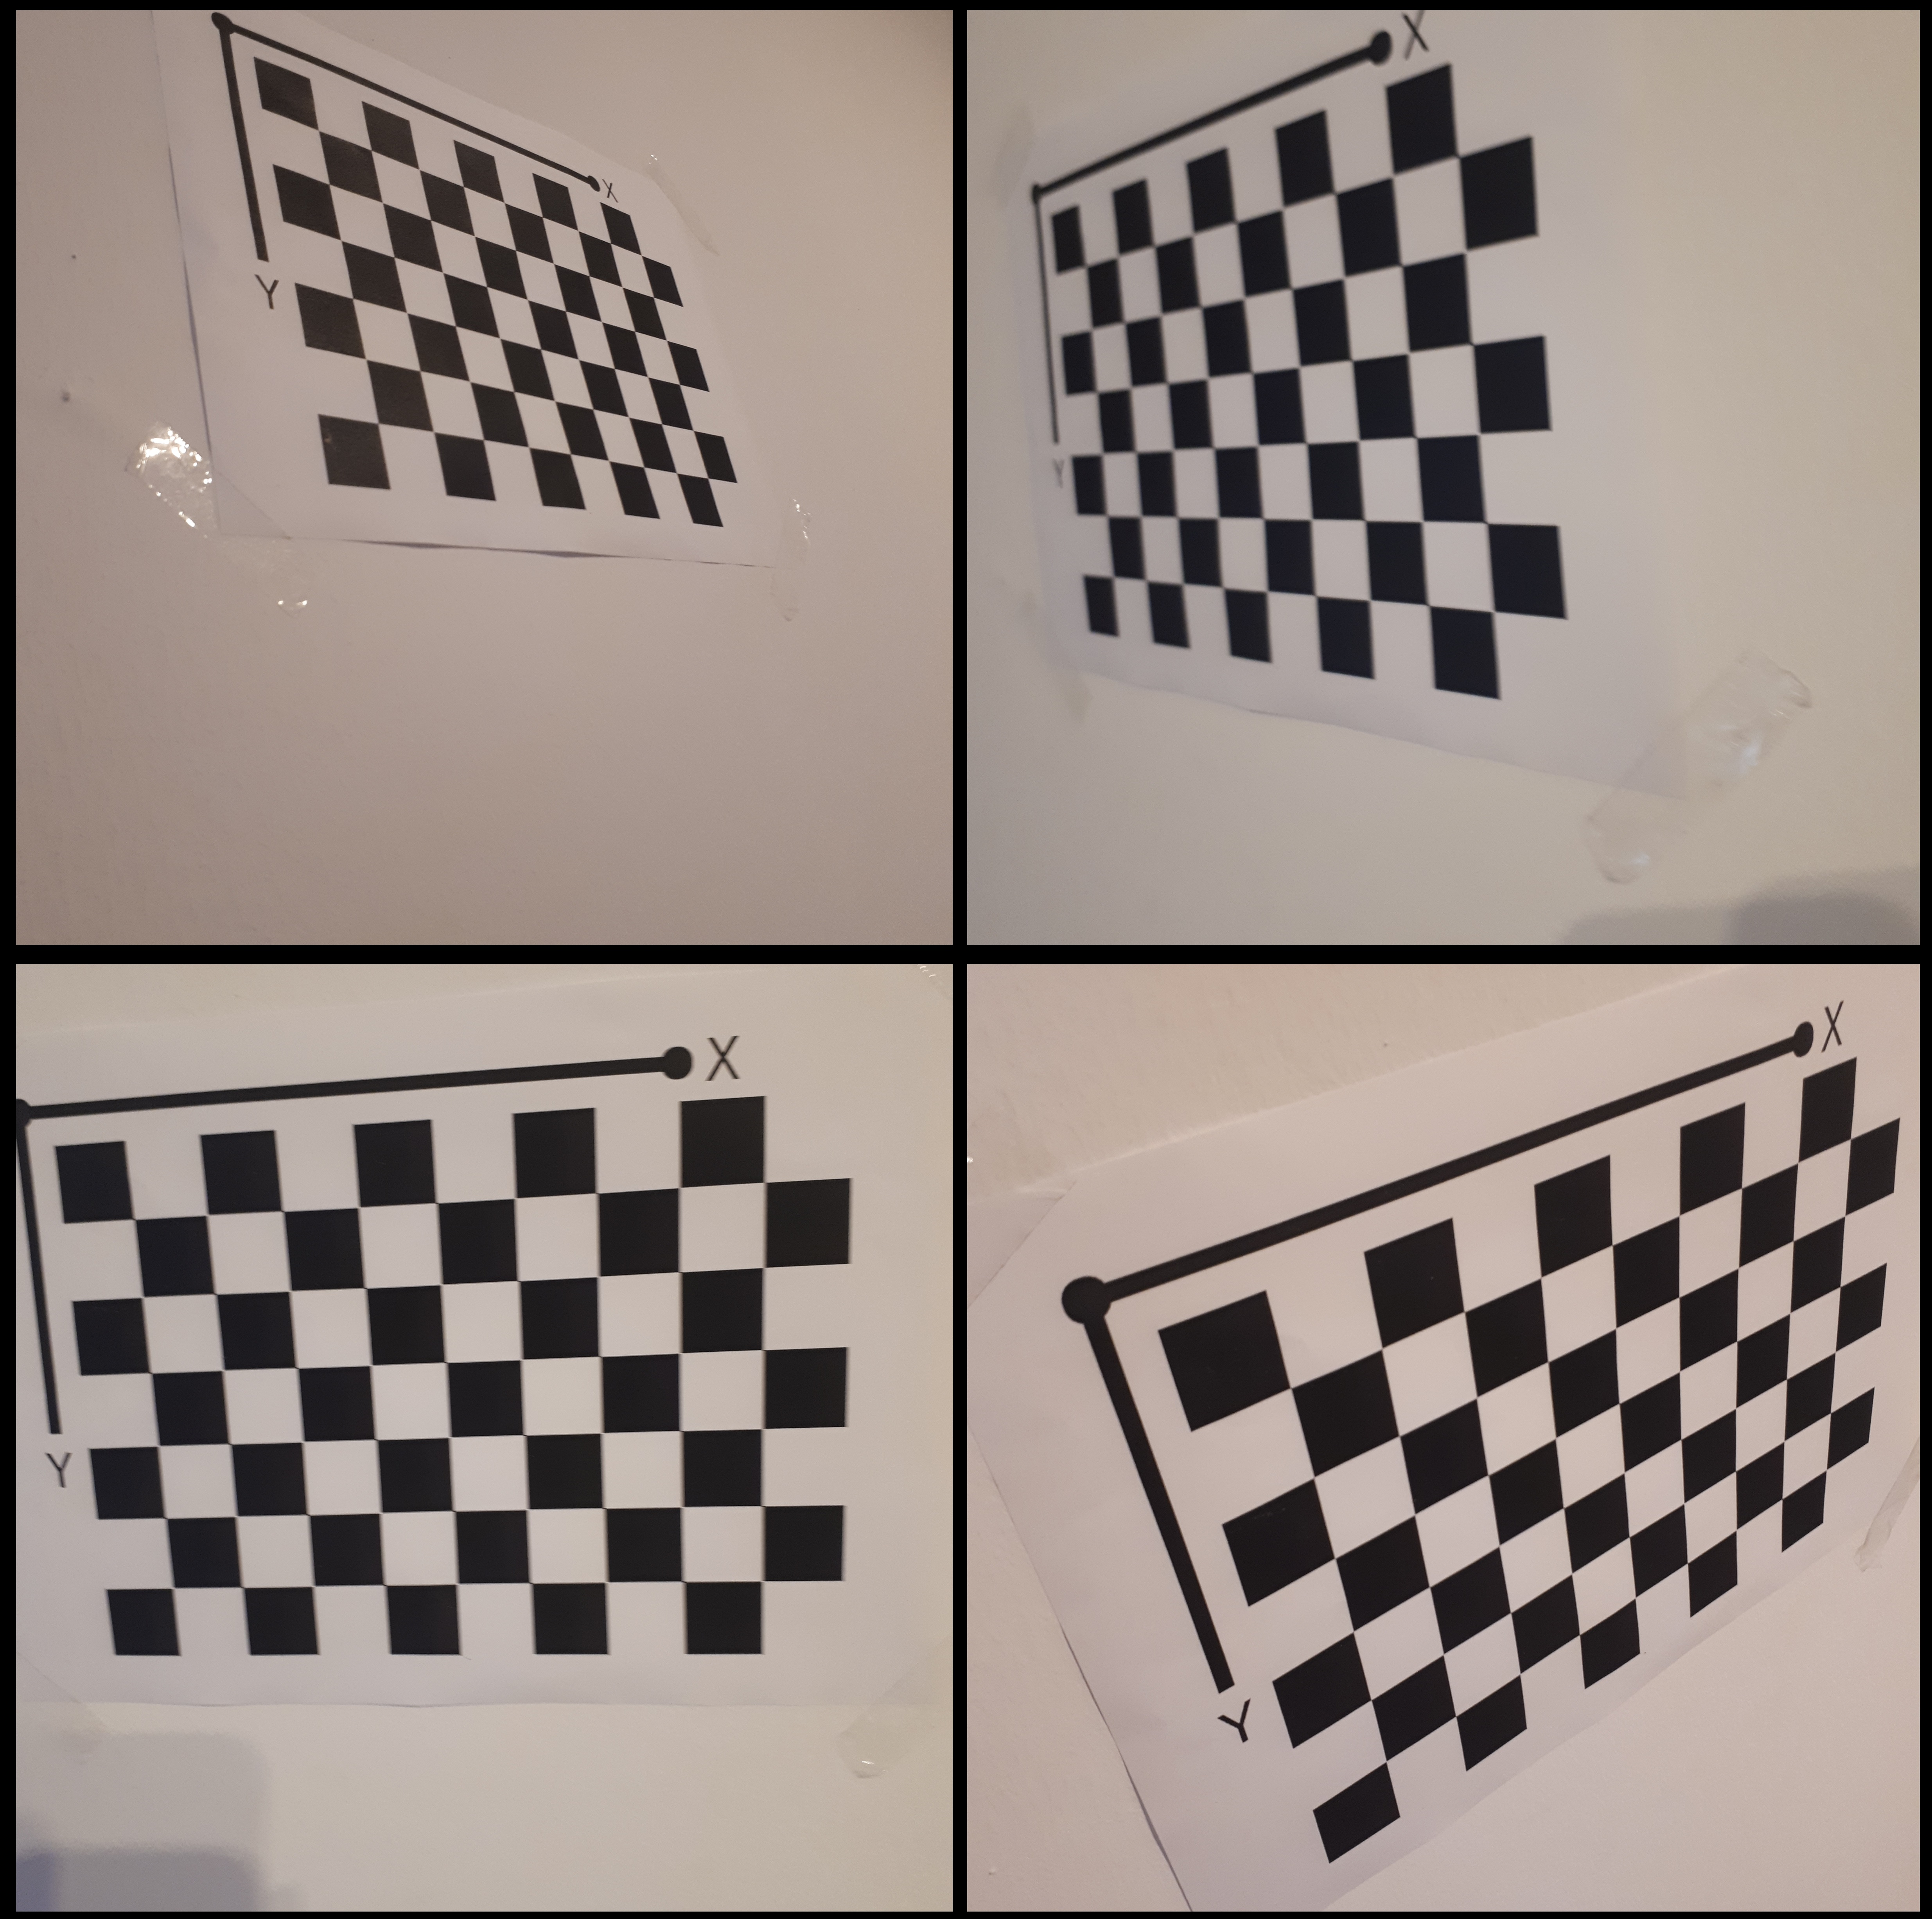
\includegraphics[scale=0.05]{Figures/Kalib1.jpg}
    \caption{Bilder des Kalibrierungsboards}
\end{figure}

Aus diesen Bildern und der Information wie groß die Abstände der einzelnen Quadrate sind ermittelt die Applikation extrinsische und intrinsische Kameraparameter. Diese können als CameraParameters Objekt gespeichert und an anderer Stelle wieder geladen werden. Das CameraParamters enthält viele Informationen über die Kamera und die Kalibrierung. Von besonderer Bedeutung für diesen Einsatzweck sind hier die Einträge RadialDistortion und TangentialDistortion, welche für das Entzerren des Bildes wichtig sind. Außerdem wird die IntrinsicMatrix benötigt um aus der Fundamentalmatrix die Essentielle Matrix zu berechnen. \cite{Mathworksa}

\subsection{Schätzen der Fundamentalmatrix}
\label{sec:Schätzen der Fundamentalmatrix}
Die Fundamentalmatrix ist eine Matrix, welche die Geometrie zweier Kameras zueinander sowie deren intrinsische Parameter beschreibt. Sie stellt die algebraische Repräsentation der Epipolargeometrie dar.\cite{Richard2000}

\subparagraph{Epipolargeometrie}
Die Epipolargeometrie liefert eine geometrische Beschreibung für zwei Kameraperspektiven auf einen Punkt in der Realität. Der Vorteil dieses Modells im Gegensatz zu anderen Modellen wie der Standardstereogeometrie ist, dass die Kameras eine beliebige Brennweite haben können und sie nicht in einer Ebene liegen müssen. Dieses Modell passt also gut zur gestellten Aufgabe, da das Objekt von vielen unterschiedlichen frei positionierten Kamerastandpunkten aufgenommen wird.
\begin{figure}[ht]
    \centering
    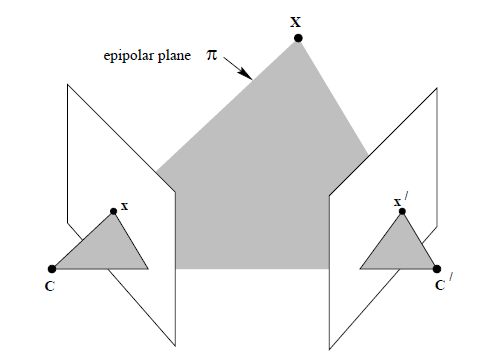
\includegraphics[scale=0.75]{Figures/Epipolargeomtrie.PNG}
    \caption{Epipolargeometrie \cite{Richard2000}}
\end{figure}
C und C’ sind hier die optischen Zentren der Kameras. Sie blicken auf einen Punkt X in der realen Welt. Die Ebene die durch die Punkte C, C’ und X aufgespannt wird nennt sich Epiolarebene. Die Punkte x und x’, die auf die Bildebene projiziert werden, liegen ebenfalls auf dieser Ebene. Die Schnittlinien zwischen der Epipolarebene sowie den Bildebenen sind die Epipolarlinien. Korrespondierene Punkte müssen auf den jeweiligen Epipolarlinien liegen. Da ein anderer Punkt X eine andere Epipolarebene aufspannen würde, wären dessen Epipolarlinien auch andere. Die Schnittpunkte der Basislinie (C – C’) mit der Bildebene sind die Epipole. Alle Epipolarlinien verlaufen durch die Epipole. \cite{Richard2000}

\subparagraph{Fundamentalmatrix}
Aus der Epipolargeometrie lässt sich die Fundamentalmatrix herleiten, die Informationen über die extrinsischen Kameraparameter (Position, Orientierung) sowie die Intrinsischen Parameter (Brennweite, Bildhauptpunkt) enthält. Sie stellt die algebraische Repräsentation der Epipolargeometrie dar. Die Fundamentalmatrix ist eine 3x3 Matrix und hat immer den Rang 2. Hat man einen korrespondierenden Punkt auf 2 Bildebenen x und x’, so muss mit der Fundamentalmatrix F gelten:
$$x'Fx = 0$$
Dies wird bei der Berechnung der Fundamentalmatrix noch wichtig. Sie wird über einen einen Datensatz an möglichen Punktkorrespondenzen über den 8-Punkte Algorithmus geschätzt. \cite{Richard2000}

\subparagraph{8-Punkte Algorithmus}
Der 8-Punkte Algorithmus ist der einfachste Algorithmus zum Schätzen der Fundamentalmatrix. Im speziellen wird hier der normalisierte 8-Punkte Algorithmus betrachtet, da die Normalisierung der Punkte zu besseren Ergebnissen führt.
Bei der Normalisierung werden die Punkte so verschoben, dass ihr Mittelpunkt der Nullpunkt ist, und zusätzlich so skaliert, dass deren Abstand im quadratischen Mittel sqrt(2) vom Nullpunkt entspricht. Die Normierung führt dazu dass das zu lösende Problem des 8-Punkte Algorithmus wesentlich besser konditioniert ist.
Der 8-Punkte Algorithmus basiert auf der Eigenschaft:
$$[x,y,1] F [x',y',1] = 0$$
Ausgeschrieben entspricht dies folgendem Gleichungssystem:
\\
$$x'xf_{11} + x'yf_{12}  + x'f_{13} + y'xf_{21} + y'yf_{22} + y'f_{23} + xf_{31} + yf_{32} + f_{33} = 0$$
Diese Gleichung kann nun umgestellt werden sodass
\\
$$Af = 0$$
\\
mit
$$A = [x'x, x'y, x', y'x, y'y, y', x,y,1]$$
und
$$f = [f11,f12,f13,f21,f22,f23,f31,f32,f33]^T$$
Die Fundamentalmatrix hat trotz ihrer 9 Einträge lediglich 7 Freiheitsgrade, da sie nur bis auf ihren Skalierungsfaktor definiert ist und die Bedingung an sie gestellt wird dass ihre Determinante 0 ist. Daher kann mit mindestens 8 korrespondierenden Punktepaaren über die Singulärwertzerlegung eine Lösung für f gefunden werden. Diese ist der Singulärvektor der zum kleinsten Singulärwert von A korrespondiert. Die Singulärwerte befinden sich in der Diagonalmatrix D. Zerlegt man A mittels Singulärwertzerlegung in UDV, so ist die Lösung in der letzten Spalte von V zu finden.
$$f = \begin{pmatrix} V_{1,end} & V_{2,end} & V_{3,end}\\V_{4,end} & V_{5,end} & V_{6,end} \\V_{7,end} & V_{8,end} & V_{9,end} \end{pmatrix} $$

Für eine ideale Fundamentalmatrix müsste nach einer Singulärwertzerlegung von f gelten:
$$D_{ideal} = \begin{pmatrix} \sigma_1 & 0 & 0\\0 & \sigma_2 & 0 \\0 & 0 & 0 \end{pmatrix}$$
Dies wird in der Realität nicht vorkommen, da hier mit diskreten Pixeln gearbeitet wird und so nie die ideale Fundamentalmatrix berechnet werden kann.
$$D_{real} = \begin{pmatrix} \sigma_1 & 0 & 0\\0 & \sigma_2 & 0 \\0 & 0 & \sigma_3 \end{pmatrix}$$
Daher wird der dritte Diagonaleintrag von D auf 0 gesetzt und die Fundamentalmatrix aus den drei Matrizen aus der Zerlegung erneut berechnet. \cite{Richard2000} \cite{Schreer2005}

\subparagraph{Schätzen der Fundamentalmatrix mittels RANSAC}
Um eine möglichst gute Fundamentalmatrix zu erhalten, wird der RANSAC Algorithmus verwendet. Er nimmt sich aus der Menge der korrespondierenden Punktepaare 8 zufälllige Punkte heraus. Damit wird über den 8-Punkte Algorithmus eine Fundamentalmatrix berechnet. Um die Güte dieser Fundamentalmatrix zu prüfen wird nun ermittelt wie viele korrespondierende Punktepaare zu der berechneten Fundamentalmatrix passen. Dazu wird die Sampson Distanz ermittelt, welche sich wie folgt berechnet.

$$d =  \dfrac{(x'^TFx)^2}{(Fx)^2_1 + (Fx)^2_2 + (Fx')^2_1) + (Fx')^2_2}$$

$(Fx)^2_j$ beschreibt hier den j-ten Eintrag im Vektor $(Fx)^2$.

Liegt ein korrespondierendes Punktepaar unter einem gewissen Schwellwert, zählt er als Inlier und gilt als zum Modell passend. Diese Berechnung wird über viele Iterationen mit immer zufällig ausgewählten Punkten für die Berechnung der Fundamentalmatrix wiederholt. Die Fundamentalmatrix die die meisten Inlier hat, deren Modell also am besten zu den Daten passt wird jeweils gespeichert. Wurden alle Iterationen durchlaufen, wird die Fundamentalmatrix erneut über den 8-Punkte Algorithmus mit allen Inliern der besten Fundamentalmatrix berechnet. \cite{Richard2000} \cite{Mathworksb}

\begin{figure}[ht]
    \centering
    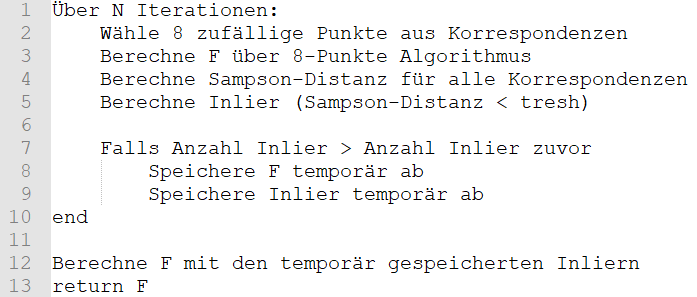
\includegraphics[scale=0.75]{Figures/PseudocodeRansac.PNG}
    \caption{Pseudocode RANSAC für Fundamentalmatrix}
\end{figure}

\subsection{Schätzen der Kamerapose aus der Fundamentalmatrix}
\label{sec:Schätzen der Kamerapose aus der Fundamentalmatrix}
Um aus der Fundamentalmatrix die Kamerapose zu schätzen, muss diese zunächst in die Essenzielle Matrix umgewandelt werden. Diese steht in enger Verbindung zur Fundamentalmatrix, allerdings hat sie nur 5 Freiheitsgrade, nämlich 3 für die Rotation und 2 für die Translation (auch hier ohne Skalierungsfaktor). Um aus der Fundamentalmatrix die Essenzielle Matrix zu berechnen, muss diese mit der Intrinsischen Matrix des CameraParams Objekt, welches aus der Kalibrierung generiert wurde, multipliziert werden. Die Intrinsische Matrix enthält die Informationen über die Brennweite sowie den Bildhauptpunkt. Da hier alle Bilder mit der gleichen Kamera aufgenommen wurden, wird die Fundamentalmatrix zwei mal mit der gleichen intrinsischen Matrix multipliziert.
$$E = I' * F * I$$
Um aus der Essenziellen Matrix die Rotation und Translation zu erhalten wird E mittels Singulärwertzerlegung in die Matrizen U,D und V zerlegt.
$$E = UDV$$
Zusätzlich werden die Matrizen W und Z benötigt:
$$W = \begin{pmatrix} 0 & -1 & 0 \\1 & 0 & 0\\0 & 0 & 1\end{pmatrix}$$
$$Z = \begin{pmatrix} 0 & 1 & 0 \\-1 & 0 & 0\\0 & 0 & 0\end{pmatrix}$$

Dabei ist W eine Rotationsmatrix und Z schiefsymmetrisch. Hier ergeben sich nun 2 mögliche Lösungen für die Rotationsmatrix:
$$R_1 = UW'V'$$
$$R_2 = UWV'$$
Beide Lösungen sind gültig und müssen später verifiziert werden. Der Translationsvektor lässt sich einfach aus der dritten Spalte von U ablesen oder durch die Formel:
$$t = UZU'$$
ermitteln. Aufgrund des fehlenden Skalierungsfaktors könnte die mögliche Lösung aber auch
t = -t
sein. Daher ergeben sich für die Kamerapose nun 4 mögliche Lösungen:
$$R_1, t$$
$$R_1, -t$$
$$R_2, t$$
$$R_2, -t$$
Um zu prüfen welche Kameraposen die richtigen sind wird nun für jede Kombination eine Triangulierung der Inlier aus der Fundamentalmatrix Berechnung durchgeführt. Die erste Kamera befindet sich dabei im Nullpunkt mit der Orientierung eye(3), die zweite hat jeweils eine der vier möglichen Lösungen. Die genaue Vorgehensweise der Triangulation wird im nächsten Kapitel beschrieben. Bei der der Realität entsprechende Lösung, müssten (fast) alle in den 3D Raum triangulierten Punkte vor beiden Kameras liegen, bei den falschen Lösungen müssten sie hinter mindestens einer Kamera liegen. Zum Schluss werden die als richtig ermittelte Lösung noch in das Koordinatensystem der ersten Kamera überführt, indem die Rotationsmatrix transponiert wird und diese auf den Translationsvektor multipliziert wird. Dann werden sie als Pose der zweiten Kamera relativ zur ersten zurückgegeben. \cite{Richard2000} \cite{LTH2013}
\begin{figure}[ht]
    \centering
    \includegraphics[scale=0.6]{Figures/validierungDerLosungen.PNG}
    \caption{4 mögliche Lösungen \cite{LTH2013}}
\end{figure}

\subsection{Triangulation}
\label{sec:Triangulation}
Die Triangulation ist eine Technik die aus Bildpunkten auf der Bildebene zweier Kameras Punkte im 3D Raum errechnet. Dafür wird eine Kameramatrix oder Projektionsmatrix benötigt. Sie ist eine 4x3 Matrix und enthält die interenen und externen Kameraparameter einer Kamera.  Sie beschreibt die Projektion eines Punktes in der realen Welt auf die Bildebene der Kamera.
$$ \begin{pmatrix} x\\y\\w \end{pmatrix} =  \begin{pmatrix} p_{11} & p_{12} & p_{13} & p_{14}\\  p_{21} & p_{22} & p_{23} & p_{24} \\  p_{31} & p_{32} & p_{33} & p_{34}  \end{pmatrix} \begin{pmatrix} X\\Y\\Z\\W \end{pmatrix}$$
Hier wird die Datenstruktur CameraMatrix von Matlab verwendet, die aus den Kameraparametern sowie den zuvor berechneten Kameraposen die Kameramatrix errechnet.
Für die Triangulation wird die Form
$$x = PX$$
umgestellt in
$$AX = 0$$
A wird nach folgender Vorschrift aufgebaut:
$$A = \begin{pmatrix} xp^{3T} - p^{1T} \\ yp^{3T} - p^{2T} \\ x'p'^{3T} - p'^{1T} \\ y'p'^{3T} - p'^{T} \end{pmatrix}$$

Mit $p^i$ wird hier die i-te Zeile der Kameramatrix P bezeichnet. Die Punke x,y und x’,y’ sind die korrespondierenden Bildpunkte in Pixeln. Wird nur zwischen zwei Kameras trianguliert, so kann A genau wie in der Formel erstellt werden. Wird zwischen mehreren Kameras trianguliert, wie am Ende des Gesamtalgorithmus so kann A analog zur oberen Formel aufgebaut werden, mit jeweils 2 weiteren Zeilen für jede weitere Kamera.
Die Lösung für X wird über die homogene Methode ermittelt, indem A mittels Singulärwertzerlegung wieder in die 3 Matrizen U,D und V zerlegt wird. Die Lösung ist hier wieder korrespondierend zum kleinsten Singulärwert und daher, bei absteigender Größe der Singulärwerte in D,  in der letzten Spalte von V zu finden. \cite{Richard2000}
$$A = UDV$$
$$X = V(end)$$

\subsection{Ergebnisse}
Mittels dieser Algorithmen sollte aus folgender Bildfolge eine Punktwolke gerechnet werden:
\begin{figure}[ht]
    \centering
    \includegraphics[scale=0.03]{Figures/Bildserie.jpg}
    \caption{Bildserie}
\end{figure}
\\
\\
\\
\\
\\
\\
Die Implementierung mit einer Korrespondenzanalyse mittels Harris Corner Detector und den Ähnlichkeitsmetriken NCC und MAE liefert folgendes Ergebnis.
\begin{figure}[ht]
    \centering
    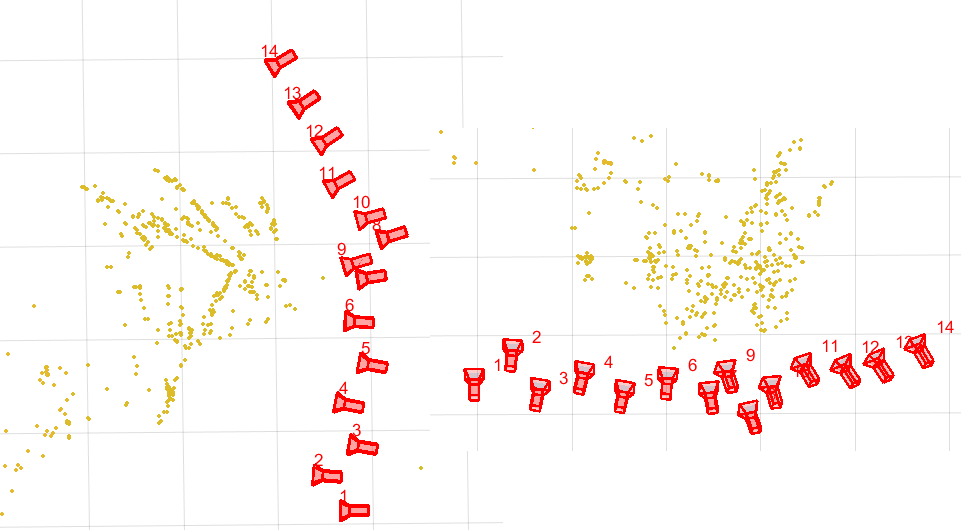
\includegraphics[scale=0.4]{Figures/ErgebnisZusammen2.png}
    \caption{Ergebnis Punktwolke}
\end{figure}
Man kann erkennen dass die Posen dem Verlauf der Kamerastandpunkte der Realität grob folgen. Allerdings sind diese mit Fehlern behaftet, sodass Sprünge zwischen den Posen auftreten die in Wirklichkeit nicht gemacht wurden. Dies wirkt sich auch auf die Qualität der Punktwolke aus. So ist die Kontur der Mauer erkennbar, doch die Punkte sind von vielen fehlerhaft rekonstruierten Punkten umgeben, welche sich aus den Fehlern der Kameraposen ergeben. Der Grund für diese Fehler liegt an der Verarbeitung zwischen Punktkorrespondenzen und der Berechnung der Fundamentalmatrix. Meist konnten hier nur wenige(10-30 von insgesamt ca. 200) Punktkorrespondenzen verwendet werden, die das Modell der Fundamentalmatrix stützen. Um dies zu testen 
wurde die Funktion 'detectSurfFeatures' aus der Matlab Computervision Toolbox zur Ermittlung der Punktkorrespondenzen verwendet. Hier war zunächst die Anzahl der gefundenen Punktkorrespondenzen höher (zw. 500 und 3000) und somit konnten auch mehr Matches verwendet werden die eine errechnete Fundamentalmatrix stützen. Je mehr Punkte (zw. 100 und 1000) für die Berechnung der Fundamentalmatrix verwendet werden, desto höher ist ihre Genauigkeit. Im Ergebnis kann man sehen dass eine weitaus dichtere Punktwolke entsteht die die Kontur der Hauswand sehr genau wiedergibt.

\begin{figure}[ht]
    \centering
    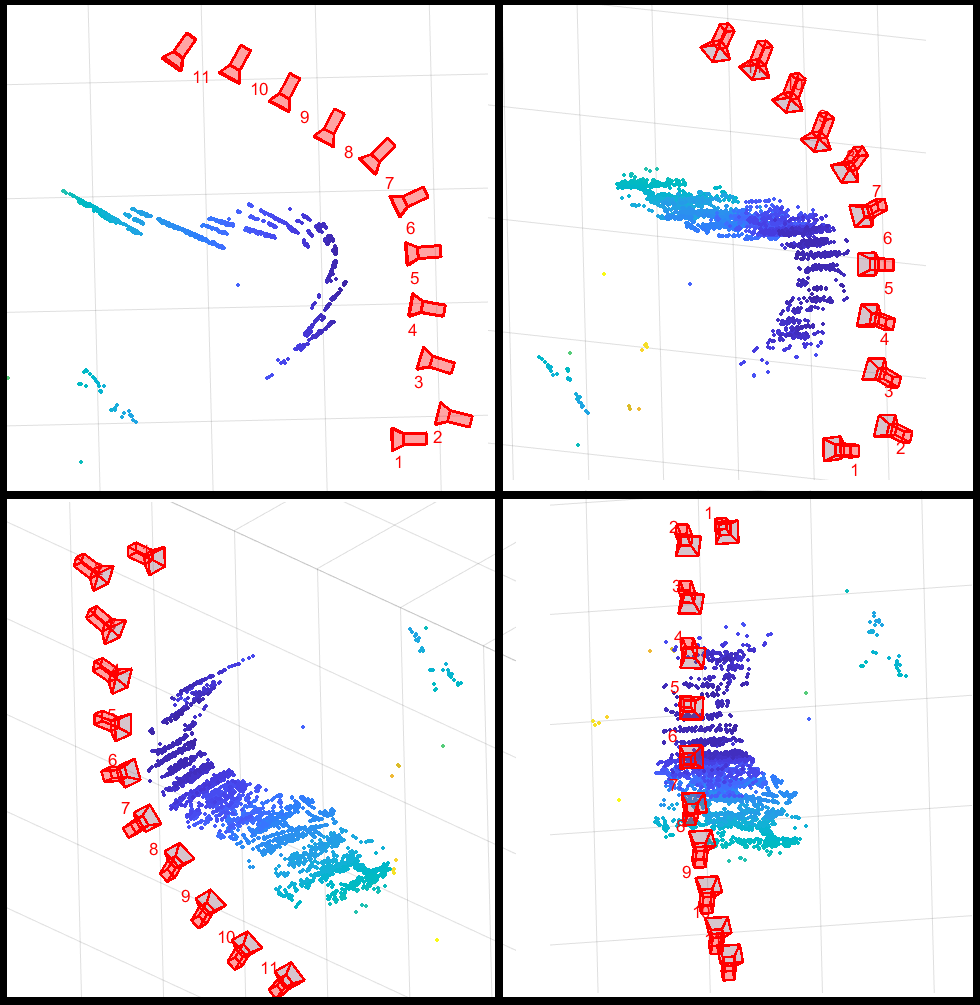
\includegraphics[scale=0.4]{Figures/ErgebnisZusammen.png}
    \caption{Ergebnis Punktwolke}
\end{figure}

\clearpage


% Appendix

\appendix
\section{Appendix}
\label{sec:appendix}


\clearpage

%------------------------------------------------------------------------------------------------------------------%
% Literaturverzeichnis
\addcontentsline{toc}{section}{Literaturverzeichnis}
\begin{spacing}{1.3}
	\printbibliography
	\clearpage
\end{spacing}

%------------------------------------------------------------------------------------------------------------------%
% Erklärung
\thispagestyle{plain}
\vspace*{\fill}
\fbox{\parbox{\linewidth}{
	\vspace{0.35cm}
	\textbf{Erklärung}
	
	\par \bigskip
	Hiermit erkläre ich gemäß der Rahmenprüfungsordnung der Hochschule München, dass ich die vorliegende Arbeit mit dem Titel ``Implementierung einer Blockchain-Anwendung zur Steigerung der Integrität von CAD-Metadaten'' selbstständig verfasst, noch nicht anderweitig für Prüfungszwecke vorgelegt, keine anderen als die angegebenen Quellen oder Hilfsmittel benutzt sowie wörtliche und sinngemäßge Zitate als solche gekennzeichnet habe.
	
	\par \bigskip
	München, den~\rule[-1mm]{3cm}{0.2mm} \hfill Unterschrift \rule[-1mm]{4cm}{0.2mm}
	\vspace{0.35cm}
}}
\vspace*{\fill}


\end{document}